% #############################################################################
% This is Chapter 5
% !TEX root = ../main.tex
% #############################################################################
% Change the Name of the Chapter i the following line
\fancychapter{Results}
%%%%%%%%%%%%%%%%%%%%%%%%%%%%%%%%%%%%%%%%%%%%%%%%%%%%%%%%%%%%%%%%%%%%%%%%
%                                                                      %
%     File: Thesis_Results.tex                                         %
%     Tex Master: Thesis.tex                                           %
%                                                                      %
%     Author: Francisco Azeredo                                        %
%     Last modified :  2 Jul 2015                                      %
%                                                                      %
%%%%%%%%%%%%%%%%%%%%%%%%%%%%%%%%%%%%%%%%%%%%%%%%%%%%%%%%%%%%%%%%%%%%%%%%
\label{chap:results}

This chapter validates the architecture and approaches developed in Chapter~\ref{chap:systemarch} through comprehensive experiments on document extraction, schema-aware retrieval, and agentic versus naive \gls{RAG} systems. We evaluate retrieval effectiveness across multiple datasets and measure answer quality using diverse similarity metrics.

\section{Information Extraction and Document Structuring}

Multiple multimodal models were tested for information extraction: PrimaLayout and PubLayNet showed promise but were insufficiently trained and produced unpredictable results. Nougat, an OCR engine that preserves document hierarchy in Markdown format, was selected for cases where PDFs lack embedded text metadata.



\section{Metadata Extraction versus Naive RAG}
\subsection{LiHua-World Dataset}
\label{subsec:LiHua-World}
The knowledge graph experiment uses the \emph{LiHua-World} corpus from \cite{fan2025minirag}: a time-indexed set of short textual records organized into weekly folders (e.g., \path{week11/20260318_1510.txt}) and topical subfolders (e.g., \path{bakery_deliver/20260531.txt}). Each file contains concise, structured messages or notes about daily events (meetings, deliveries, fitness plans, chats, travel, garden updates), often implying participants and locations. This format provides:
\begin{itemize}
    \item \textbf{Temporal signals:} timestamps encoded in filenames (YYYYMMDD\_HHMM) and dates inside texts, enabling ordering and interval reasoning.
    \item \textbf{Multi-actor context:} recurring names across files (e.g., Li Hua, Wolfgang, Jennifer) support relationship extraction.
    \item \textbf{Domain variety:} community garden, bakery deliveries, fitness training, entertainment, and travel, which stress-test entity and relation typing.
\end{itemize}

\subsection{Knowledge Graph Ingestion Pipeline}

The corpus is processed through the metadata extraction framework by performing: (1) \textbf{Entity extraction:} using LLM-guided prompts to identify normalized entities (people, organizations, locations, events); (2) \textbf{Relation extraction:} inferring semantic relationships between entities based on embedding proximity; (3) \textbf{Object creation:} creating  Weaviate objects for extracted entities with cross-references; (4) \textbf{Vectorization}:embedding textual properties for hybrid retrieval.


In this setup, answers were generated using sentence embedding model All-MiniLM-L6-v2 for retrieval and the local LLM Qwen2M for generation. The benchmark dataset consisted of 628 questions categorized as: (1) \textbf{Single}—direct factoid questions that can be answered from a single evidence source; (2) \textbf{Multi}—questions requiring multi-hop reasoning and/or temporal or causal understanding; (3) \textbf{Null}—questions with insufficient evidence.

The experiment compares knowledge-graph–aware retrieval (Mini and Light) against a naive baseline.
Figure~\ref{fig:Lihua-World} presents the results across all metrics.
\begin{figure}[H]
    \centering
    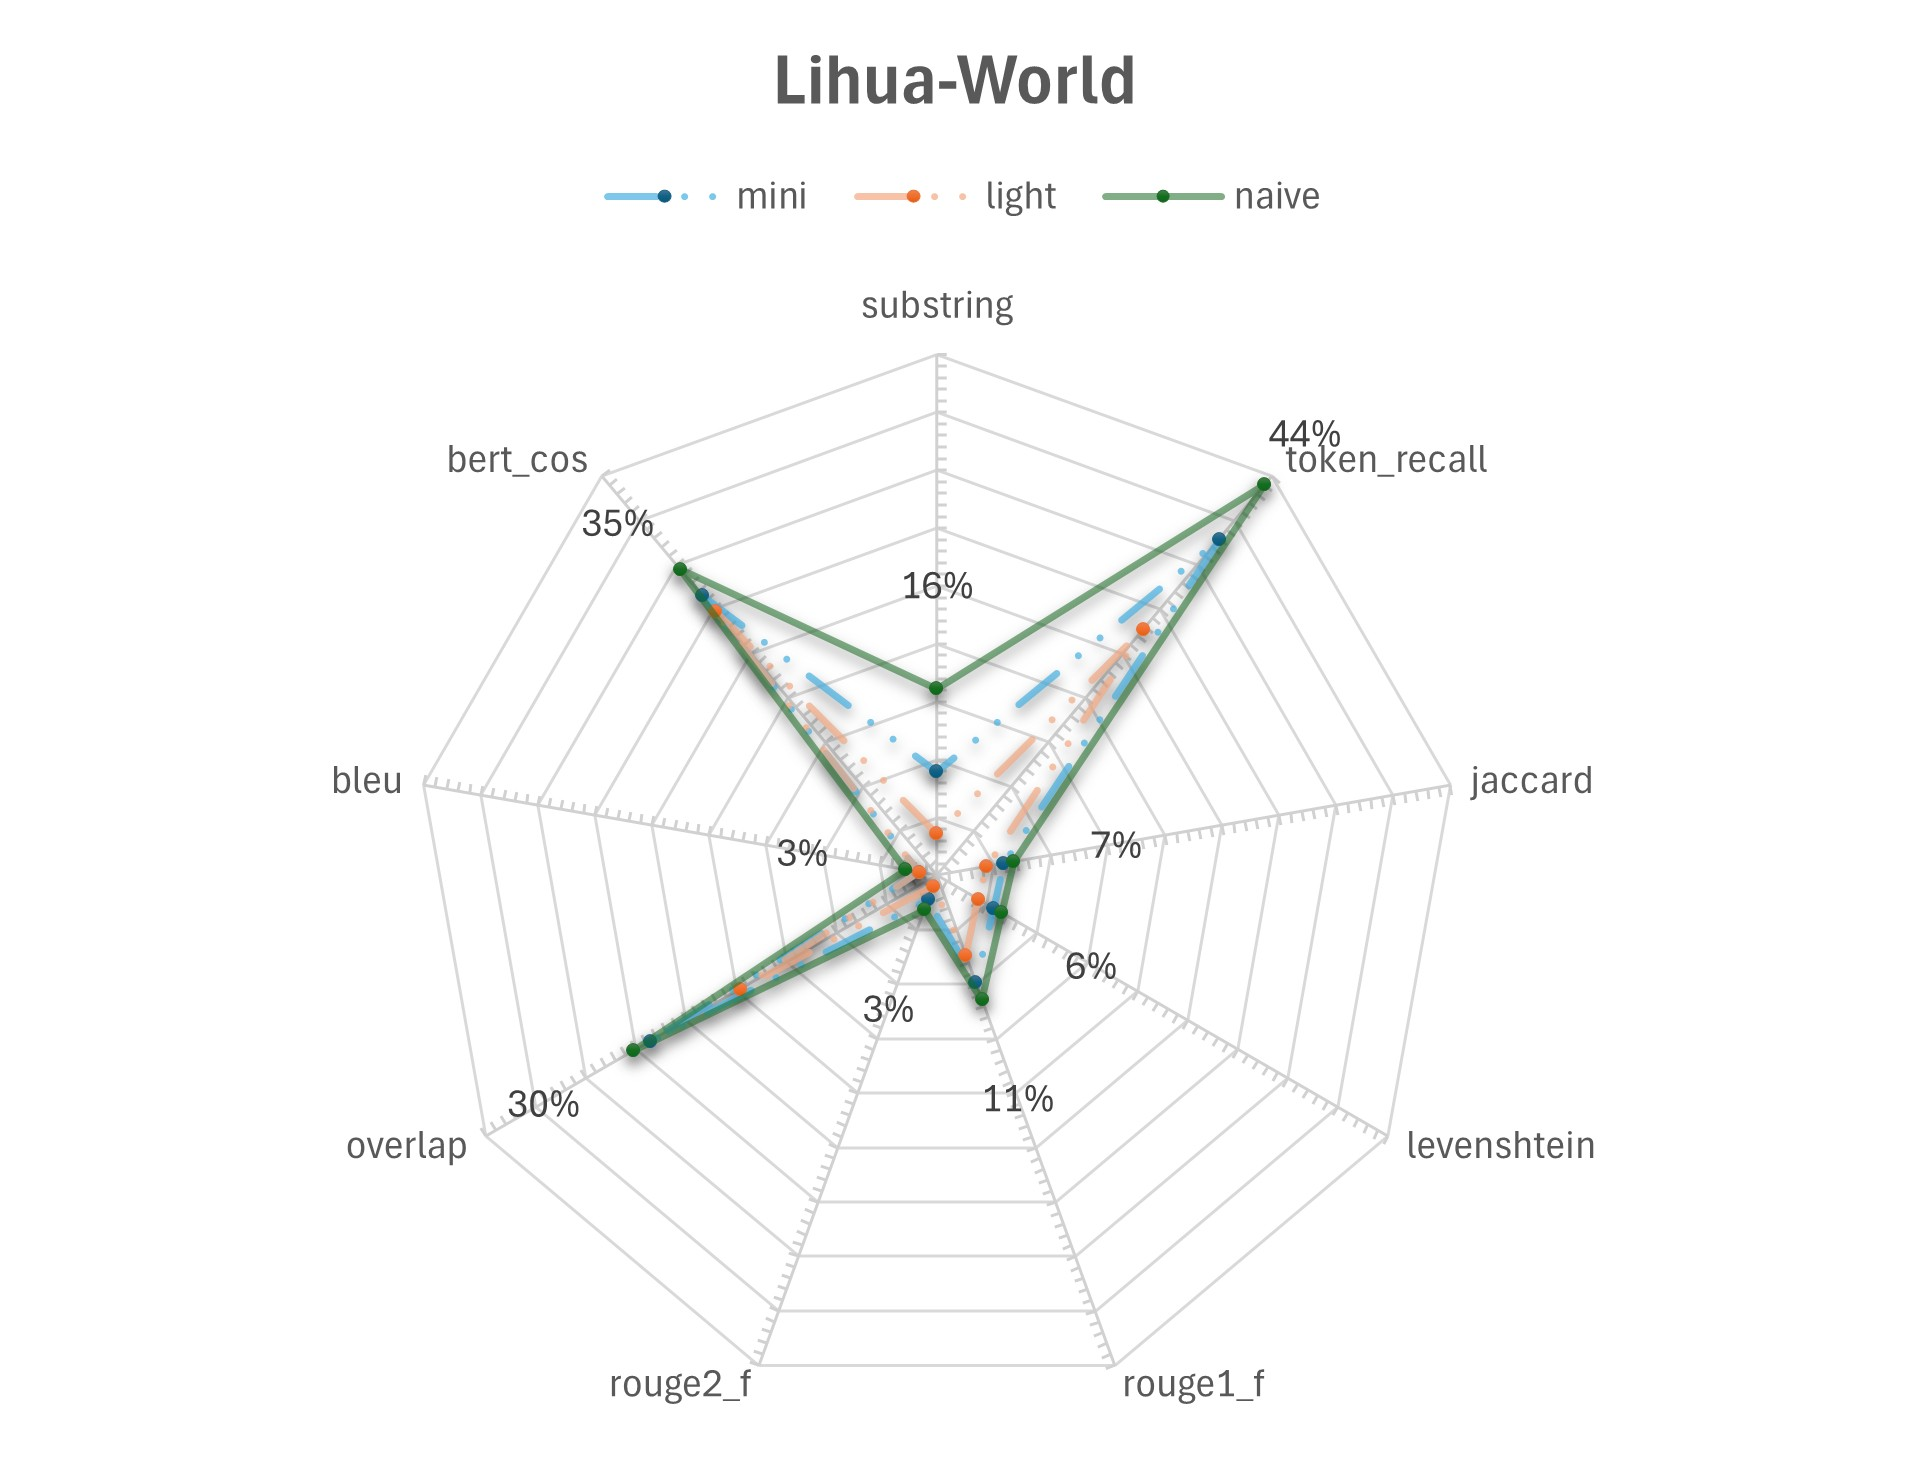
\includegraphics[width=1\linewidth]{Figures/Lihua-World.jpg}
    \caption{3 query types tested. With qwen2m as the \gls{LLM} and all-MiniLM-L6-v2 as embedding model}
    \label{fig:Lihua-World}
\end{figure}
Among the metrics, \textbf{Token Recall} achieved the highest score (44\%), and is the most relevant for this type of QA dataset.

\footnote{Note on metrics The full definitions and motivations for the evaluation metrics are provided in previous section \ref{sec:text-similarity-metrics}. Here we briefly reference the same set—lexical (Token Recall, Jaccard, Overlap), structural (Levenshtein, ROUGE, BLEU), and semantic (\gls{BERT} cosine)—and focus on interpreting the results in this experiment.}

\subsection{Semantic Similarity}
	\textbf{\gls{BERT} cosine similarity} score was moderate (35\%). This is largely due to length imbalance between short gold answers (sometimes a single token) and longer generated responses: sentence-level embeddings such as \textit{all-MiniLM-L6-v2} capture global semantics, so single-token vs. full-sentence comparisons tend to yield low cosine values.

\subsection{Lexical Accuracy}
	\textbf{Token Recall} (44\%) confirms that gold tokens are often present in predictions. The \textbf{Overlap Coefficient} (30\%) is comparatively robust to length differences, since it does not penalize extra tokens. In contrast, \textbf{Jaccard} (7\%) performs poorly when generated answers are longer, as the inflated union suppresses the overlap proportion—even for partially correct outputs.

\subsection{Structural Similarity}
	\textbf{Levenshtein} (6\%) provides a weak signal under large length differences. \textbf{ROUGE-1 F1} (11\%) and \textbf{ROUGE-2 F1} (3\%) partly mitigate this by balancing precision and recall over n-grams, although longer responses containing irrelevant tokens reduce precision. ROUGE-2 is particularly low because short gold answers rarely contain bigrams. Finally, \textbf{BLEU} (3\%)—originally designed for machine translation—over-penalizes deviations and brevity mismatches in this context, making it unsuitable for this task.

\subsection{Summary}
This experiment implemented an automated approach constructing a knowledge graph. The goal was to enable retrieval that leverages explicit entity relationships and organizational context rather than relying solely on surface-level text.

However, the results show that the current automatic knowledge graph construction fails to reliably produce a strong semantic structure for retrieval. In practice, direct embedding-based indexing using sentence transformers remains significantly faster, cheaper, and more effective for retrieval tasks, consistently outperforming the knowledge graph approach in this setup.

Profiling and structuring text with an LLM is also considerably more computationally expensive: each 200-token chunk is processed through a few-shot prompt (with many input tokens), up to three times, followed by an additional pass for entity merging and summarization. This makes large-scale knowledge graph construction costly. While using a heavier LLM could improve the quality of the knowledge graph and its retrieval performance, the resource requirements and latency increase substantially.

In summary, while knowledge graphs offer richer structure representations and could become more competitive with stronger \glspl{LLM}, current embedding models provide a more scalable and efficient solution for semantic retrieval. Future work may revisit knowledge graph approaches as the cost of \glspl{LLM} decrease and their capabilities improve.

\section{Naive \gls{RAG} versus \gls{ARAG} on Company Information}
\label{sec:expNaiveVsAgenticRAG}
This experiment aims to evaluate the effectiveness of an agentic retrieval-augmented generation (\gls{RAG}) approach compared to a naive \gls{RAG} baseline for answering context-specific questions about company information. The goal is to determine whether an agent capable of planning and reasoning over retrieved documents can provide more accurate and relevant answers than a straightforward retrieval and generation pipeline.

For this experiment, a synthetic company QA dataset was created in two automated stages:
\begin{enumerate}
        \item \textbf{Document Generation:} We synthesized 1{,}000 realistic administrative documents using  \gls{GPT}-5 via the OpenAI API. For each document, a classifiable node was sampled from a hierarchical public-sector classification (e.g., legislation, planning, HR, finance, justice, health, education) and prompted the model with the node’s description, notes, and index terms—while explicitly instructing it not to reveal the class name, both to preserve confidentiality when transmitting prompts to external APIs and to avoid label leakage. This produced a diverse set of plausible, well-structured administrative files spanning distinct legal and organizational contexts.
        \item \textbf{QA Pair Generation:} \label{subsec:qa-generation} Next, for a random subset of these documents, a second generative model (also \gls{GPT}-5) was employedto create question-answer pairs. The model was prompted with the full content of each document and instructed to generate a specific, contextually relevant question that could only be answered by reading that document, along with a precise answer based solely on its content. This ensures that each QA pair is tightly coupled to a single file and cannot be answered from general knowledge or other documents. The cost of generating 300 such QA pairs was approximately 0.85 dollars.
\end{enumerate}

This process produces the \gls{QA} benchmark used to evaluate thedeveloped \gls{RAG} systems, where each question can only be answerable by retrieving the correct company file and reasoning over its content. The dataset is well-suited for evaluating (\gls{RAG}) systems, as it necessitates both accurate retrieval and grounded answer generation.

\subsection{Vector Database Setup}
The vector database employed in this work is Weaviate. It is populated with 1000 synthetic company documents created earlier (see Section~\ref{sec:expNaiveVsAgenticRAG}) and indexed using \textit{sentence-transformers/all-MiniLM-L6-v2} embeddings. The schema is straightforward: a single class, \textit{Ficheiro} (file), with properties \texttt{text} and \texttt{file\_path}. Each document is stored as one object, with \texttt{text} vectorized (named vector \texttt{text\_vector}) to support semantic search; \texttt{file\_path} stores the document source for grounding answers. This index is employed by both the naive and agentic systems in the following experiments.

\subsection{Naive RAG and CoT Baselines}
\label{sec:naive-rag-and-cot-baseline}
The naive baseline retrieved top-ranked passages from Weaviate and produced an answer; the CoT variant used the same retrieval with a concise step-by-step hint.
For each question in the \gls{QA} dataset (generated in \ref{subsec:qa-generation}), the naive pipeline executes:
\begin{enumerate}
    \item Run a hybrid search in Weaviate (\(\alpha = 0.7\)) over \texttt{text\_vector} with the question to retrieve the top-$k$ objects containing \texttt{text} and \texttt{file\_path}.
    \item Generate a concise answer grounded in the retrieved content.
\end{enumerate}

At a high level, the naive pipeline performs a single retrieve-and-generate pass over hybrid search results in Portuguese. Variants with \texttt{qwen2.5} were tested to pick a cost-effective baseline, then the best was re-run with ChatGPT-5 to estimate an upper bound on quality. See Algorithm~\ref{alg:naive-weaviate-hybrid} (Appendix~B) for details.
The results are presented in Figure~\ref{fig:weaviate_test}.
This serves as a control: it is simpler to implement and does not require a large model for planning.
\begin{figure}
    \centering
    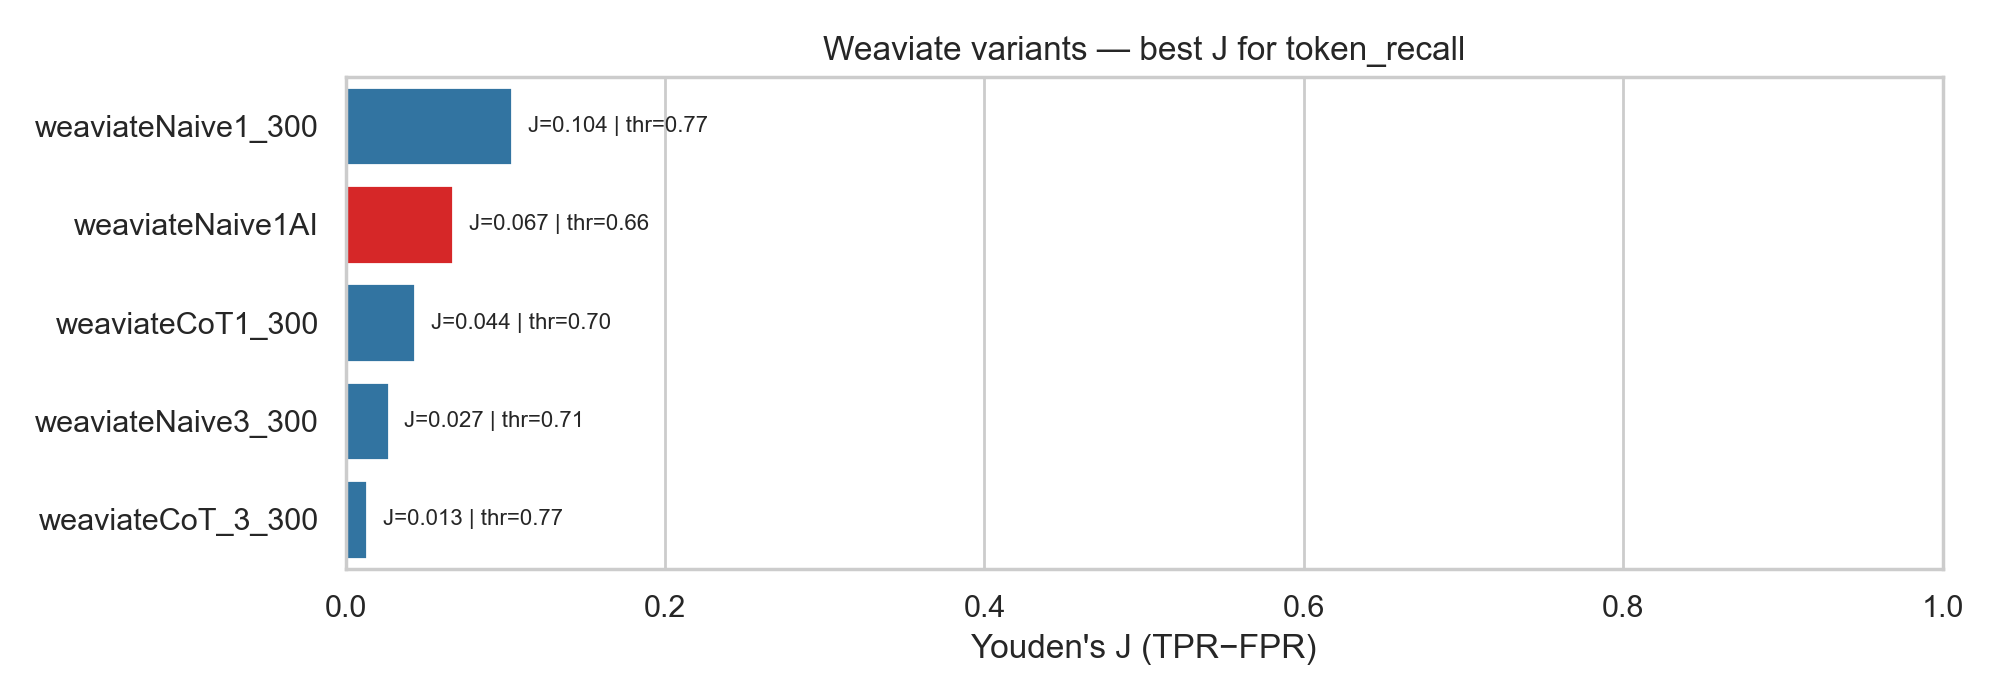
\includegraphics[width=1\linewidth]{Figures/10_weaviate_best_j_token_recall.png}
    \caption{Youden's J statistic for qualifying best naive \gls{RAG} variant. With qwen2.5m as the \gls{LLM} and all-MiniLM-L6-v2 as embedding model. And a chatgpt5 variant using best top-$k$ and prompt parameters.(k=4, prompt=naive)}
    \label{fig:weaviate_test}
\end{figure}
\subsection{Agentic RAG Setup}
\label{sec:agentic-test}

To set up the test, a \textbf{ReAct} agent was developed and connected to a Weaviate vector database via \gls{MCP} developed in this thesis~\ref{sec:weaviate-mcp-server}. Following initial trials with a local model (\texttt{qwen2.5m}) that exhibited frequent context drift—diverging from the question and producing extractive outputs—reinforcing the need for a larger context window, \textbf{ChatGPT-5} was used for planning and generation, since larger model is required to maintain multi-step reasoning within its context window.

\subsection{Agent Workflow}
For each question in the \gls{QA} dataset (generated in \ref{subsec:qa-generation}), the agent follows a ReAct loop:
\begin{enumerate}
\item \textbf{Plan:} Sketch a brief strategy to find the answer.
\item \textbf{Retrieve:} Fetch the most relevant documents.
\item \textbf{Observe \& Reflect:} Inspect the evidence and, if needed, refine the plan and retrieval.
\item \textbf{Answer:} Produce a concise response grounded in the retrieved content.
\end{enumerate}

Across \textbf{300} questions, the agent sometimes required up to \textbf{20} \gls{LLM} calls per query, with a total run cost of approximately \textbf{\$14}. While reasoning improves answer quality, it significantly increases latency and cost compared to naive \gls{RAG}.

The cost-quality trade-off can be expressed as: achieving 60.4\% retrieval rate via agentic \gls{RAG} costs approximately \textbf{\$0.047 per question}, compared to \textbf{\$0.0017} for naive \gls{RAG} at 13.8\% retrieval. This \textbf{27.6x cost increase} yields a \textbf{4.4x improvement in retrieval accuracy}, representing a favorable trade-off for scenarios where accuracy is prioritized over cost.

\section{Evaluation of Quality Metrics}
\label{sec:metric-evaluation-quality}
To evaluate answer quality, the same metrics as in the previous experiment (Section~\ref{sec:expNaiveVsAgenticRAG}) are applied. Theanalysis extends further under the hypothesis that an answer can only be correct if thecorresponding souce is correctly retrieved. This is assessed by determining the metric threshold that best separates correct from incorrect answers—i.g., the threshold that most closely aligns with successeful source retrieval. The optimal threshold is identified by maximizing Youden's J statistic, defined as the difference between true positive rate (TPR) and false positive rate (FPR).
\begin{figure}[H]
    \centering
    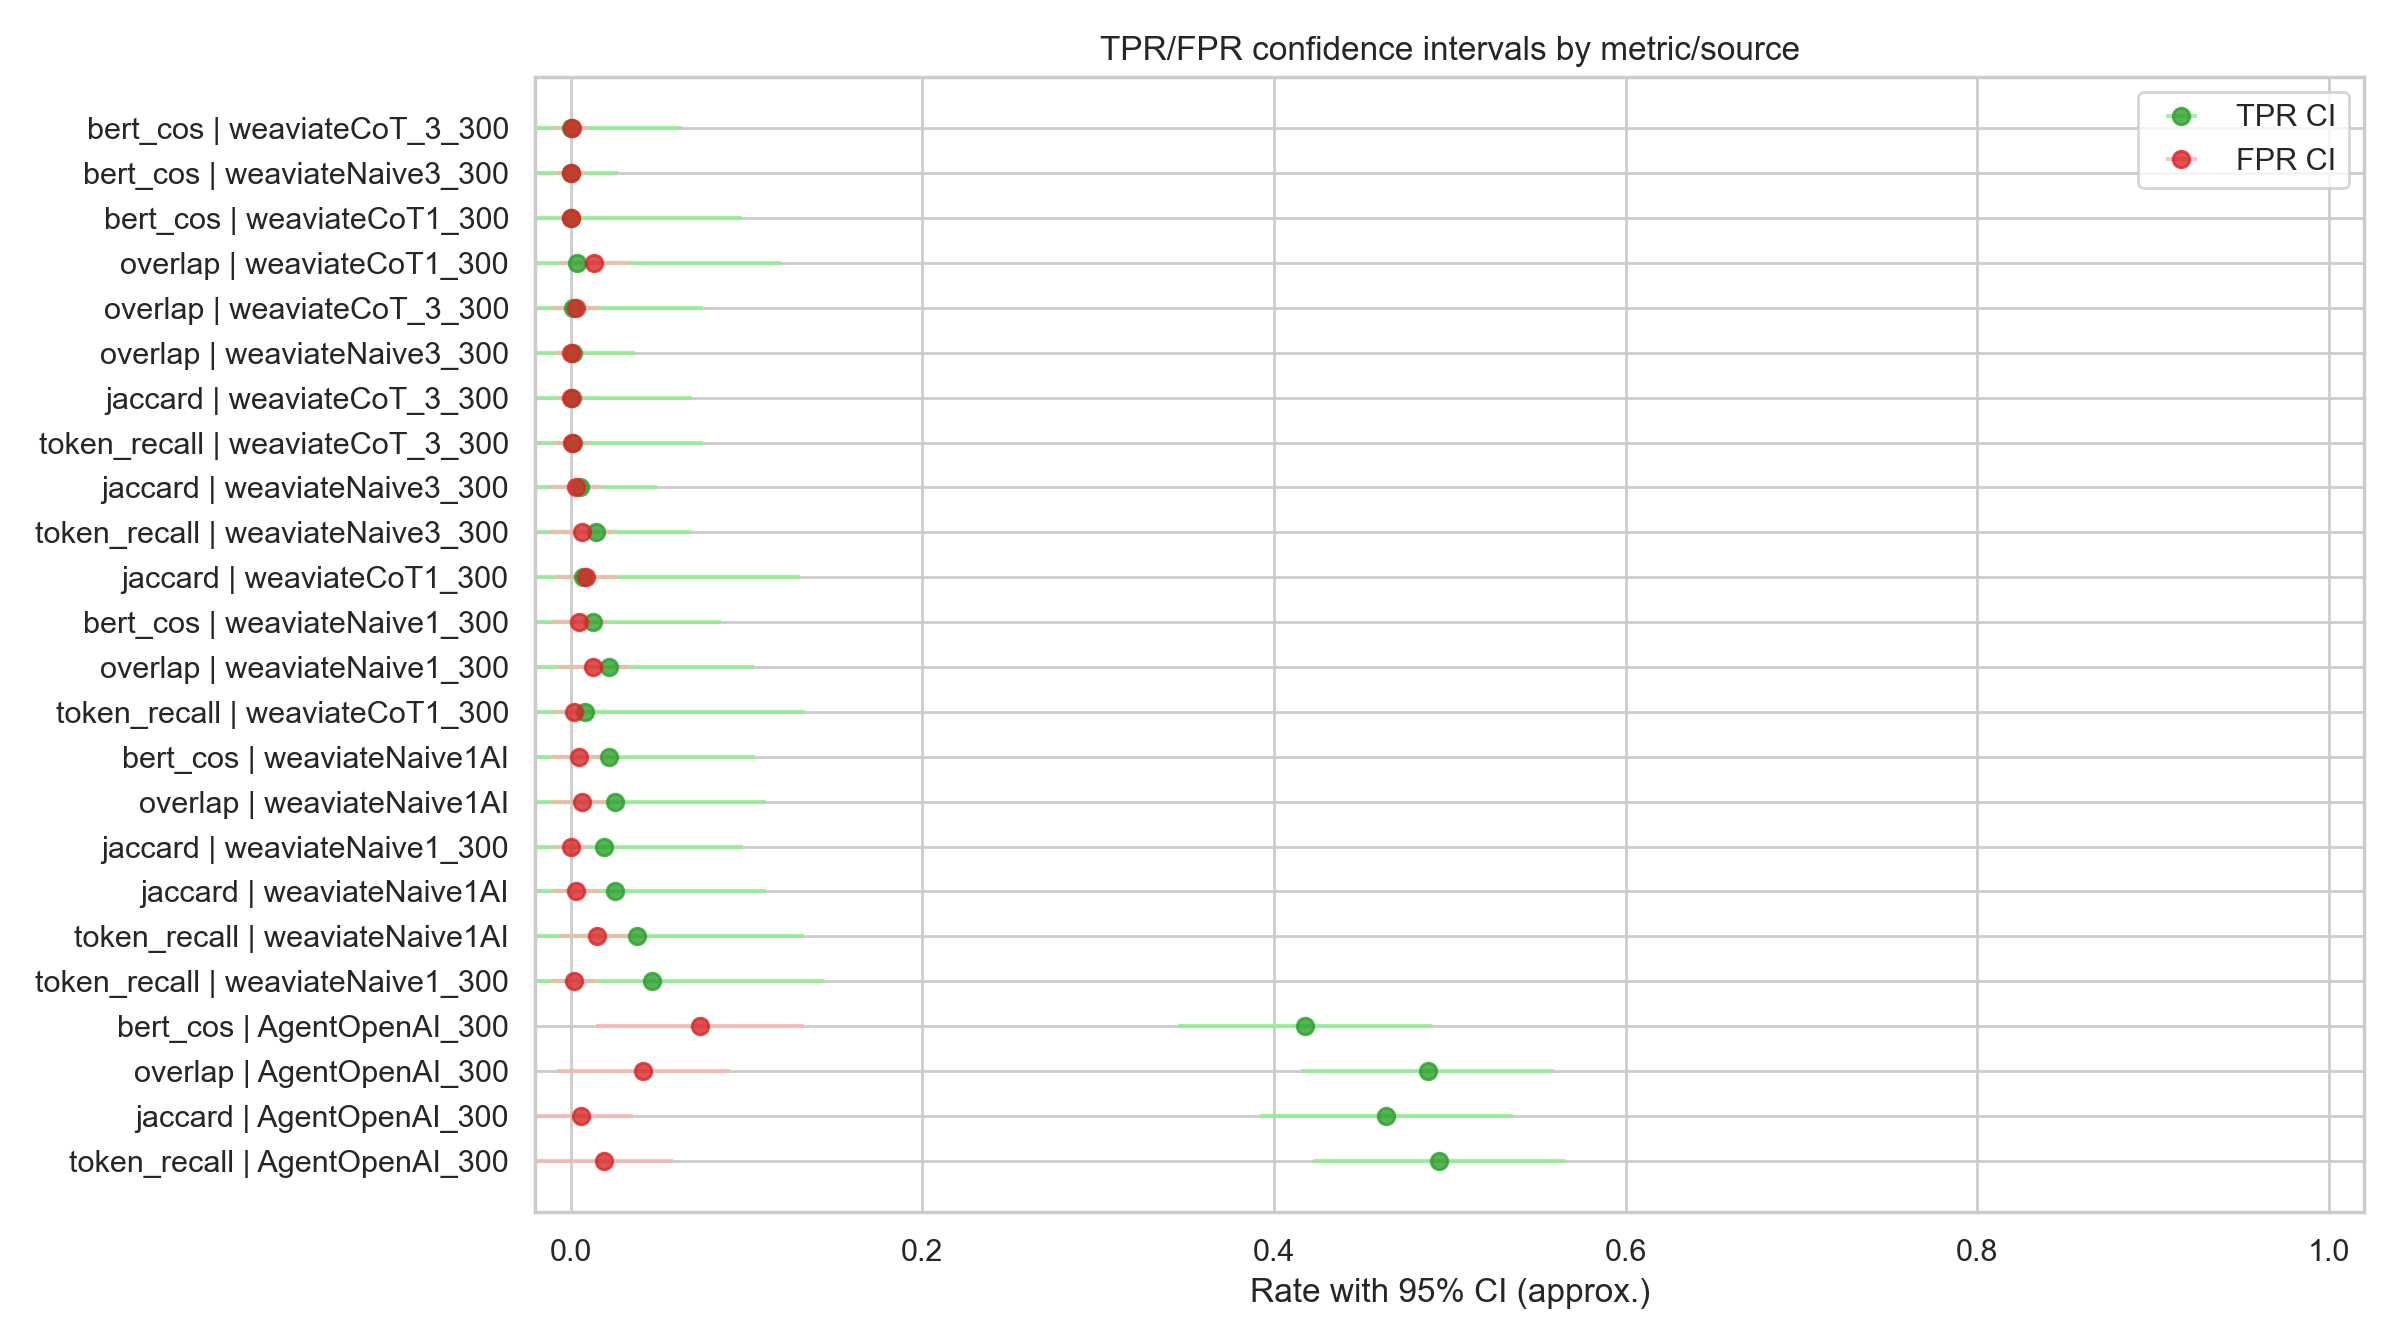
\includegraphics[width=1\linewidth]{Figures/06_tpr_fpr_confidence_intervals.png}
    \caption{confidence intervals for TPR and FPR per metric, for all source benchmark results, using the threshold that maximizes Youden's J statistic.}\label{fig:confidence-intervals}
\end{figure}

From the TPR and FPR confidence intervals (Figure~\ref{fig:confidence-intervals}), it can be observed that results obtained from the agentic RAG system have much better quality than the naive RAG system across all metrics. This indicates that the most reliable benchmark for determining thresholds using Youden's J statistic is the agentic RAG system. One contributing factor is its more balanced behavior on missed and successful retrievals. As seen from the document retrieved percentages shown in Table~\ref{tab:doc-retrieved-by-source}, the agentic RAG system substantially outperforms naive baselines: it correctly retrieves documents 60.4\% of the time, compared to 13.8\%–22.5\% for naive approaches and 5.7\%–9.4\% for chain-of-thought variants. This substantial improvement reflects the agent'sreasoning and planning capabilities, whereas the naive RAG system performs a single hybrid search.

\begin{table}[htbp]
    \centering
    \begin{tabular}{l c}
        \hline
        Source file & Correct document retrieved \\
        \hline
    AgentOpenAI\_300 & 60.4\% \\
    weaviateNaive3\_300 & 22.5\% \\
    weaviateNaive1\_300 & 13.8\% \\
    weaviateNaive1AI & 13.4\% \\
    weaviateCoT\_3\_300 & 9.4\% \\
    weaviateCoT1\_300 & 5.7\% \\
        \hline
    \end{tabular}
    \caption{Document retrieved percentage by source file}\label{tab:doc-retrieved-by-source}
\end{table}

\begin{table}[htbp]
  \centering
  \begin{tabular}{l c c c c}
    \hline
    Metric & Threshold & TPR & FPR & J \\
    \hline
    token\_recall & 0.67 & 56.7\% & 4.4\%  & 52.3\% \\
    jaccard       & 0.26 & 53.7\% & 2.0\%  & 51.7\% \\
    rouge1\_f     & 0.40 & 52.3\% & 2.7\%  & 49.7\% \\
    overlap       & 0.56 & 56.0\% & 7.7\%  & 48.3\% \\
    bleu          & 0.37 & 39.3\% & 1.3\%  & 37.9\% \\
    bert\_cos     & 0.71 & 49.0\% & 12.1\% & 36.9\% \\
    \hline
  \end{tabular}
    \caption{Best thresholds by metric (max True--False pass-rate difference) for File: AgentOpenAI\_300}\label{tab:agentopenai300-best-thresholds}
\end{table}


\subsection{Overall Metric Results}
Based on the previous subsection, the analysis indicates that the optimal metric thresholds (according to Youden's J statistic) are delivered from the agentic RAG system; these thresholds from table \ref{tab:agentopenai300-best-thresholds} are subsequently used to classify answers as correct or incorrect across benchmarks. The analysis is also narrowed to the best naive RAG variant (weaviateNaive1\_300), using qwen2.5 and OpenAI models, and the agentic RAG system (AgentOpenAI\_300). The results are presented in Figure~\ref{fig:median-metric} and Table~\ref{tab:gain-loss-reference-median}. The median metric scores are also presented for reference.
\begin{figure}
    \centering
    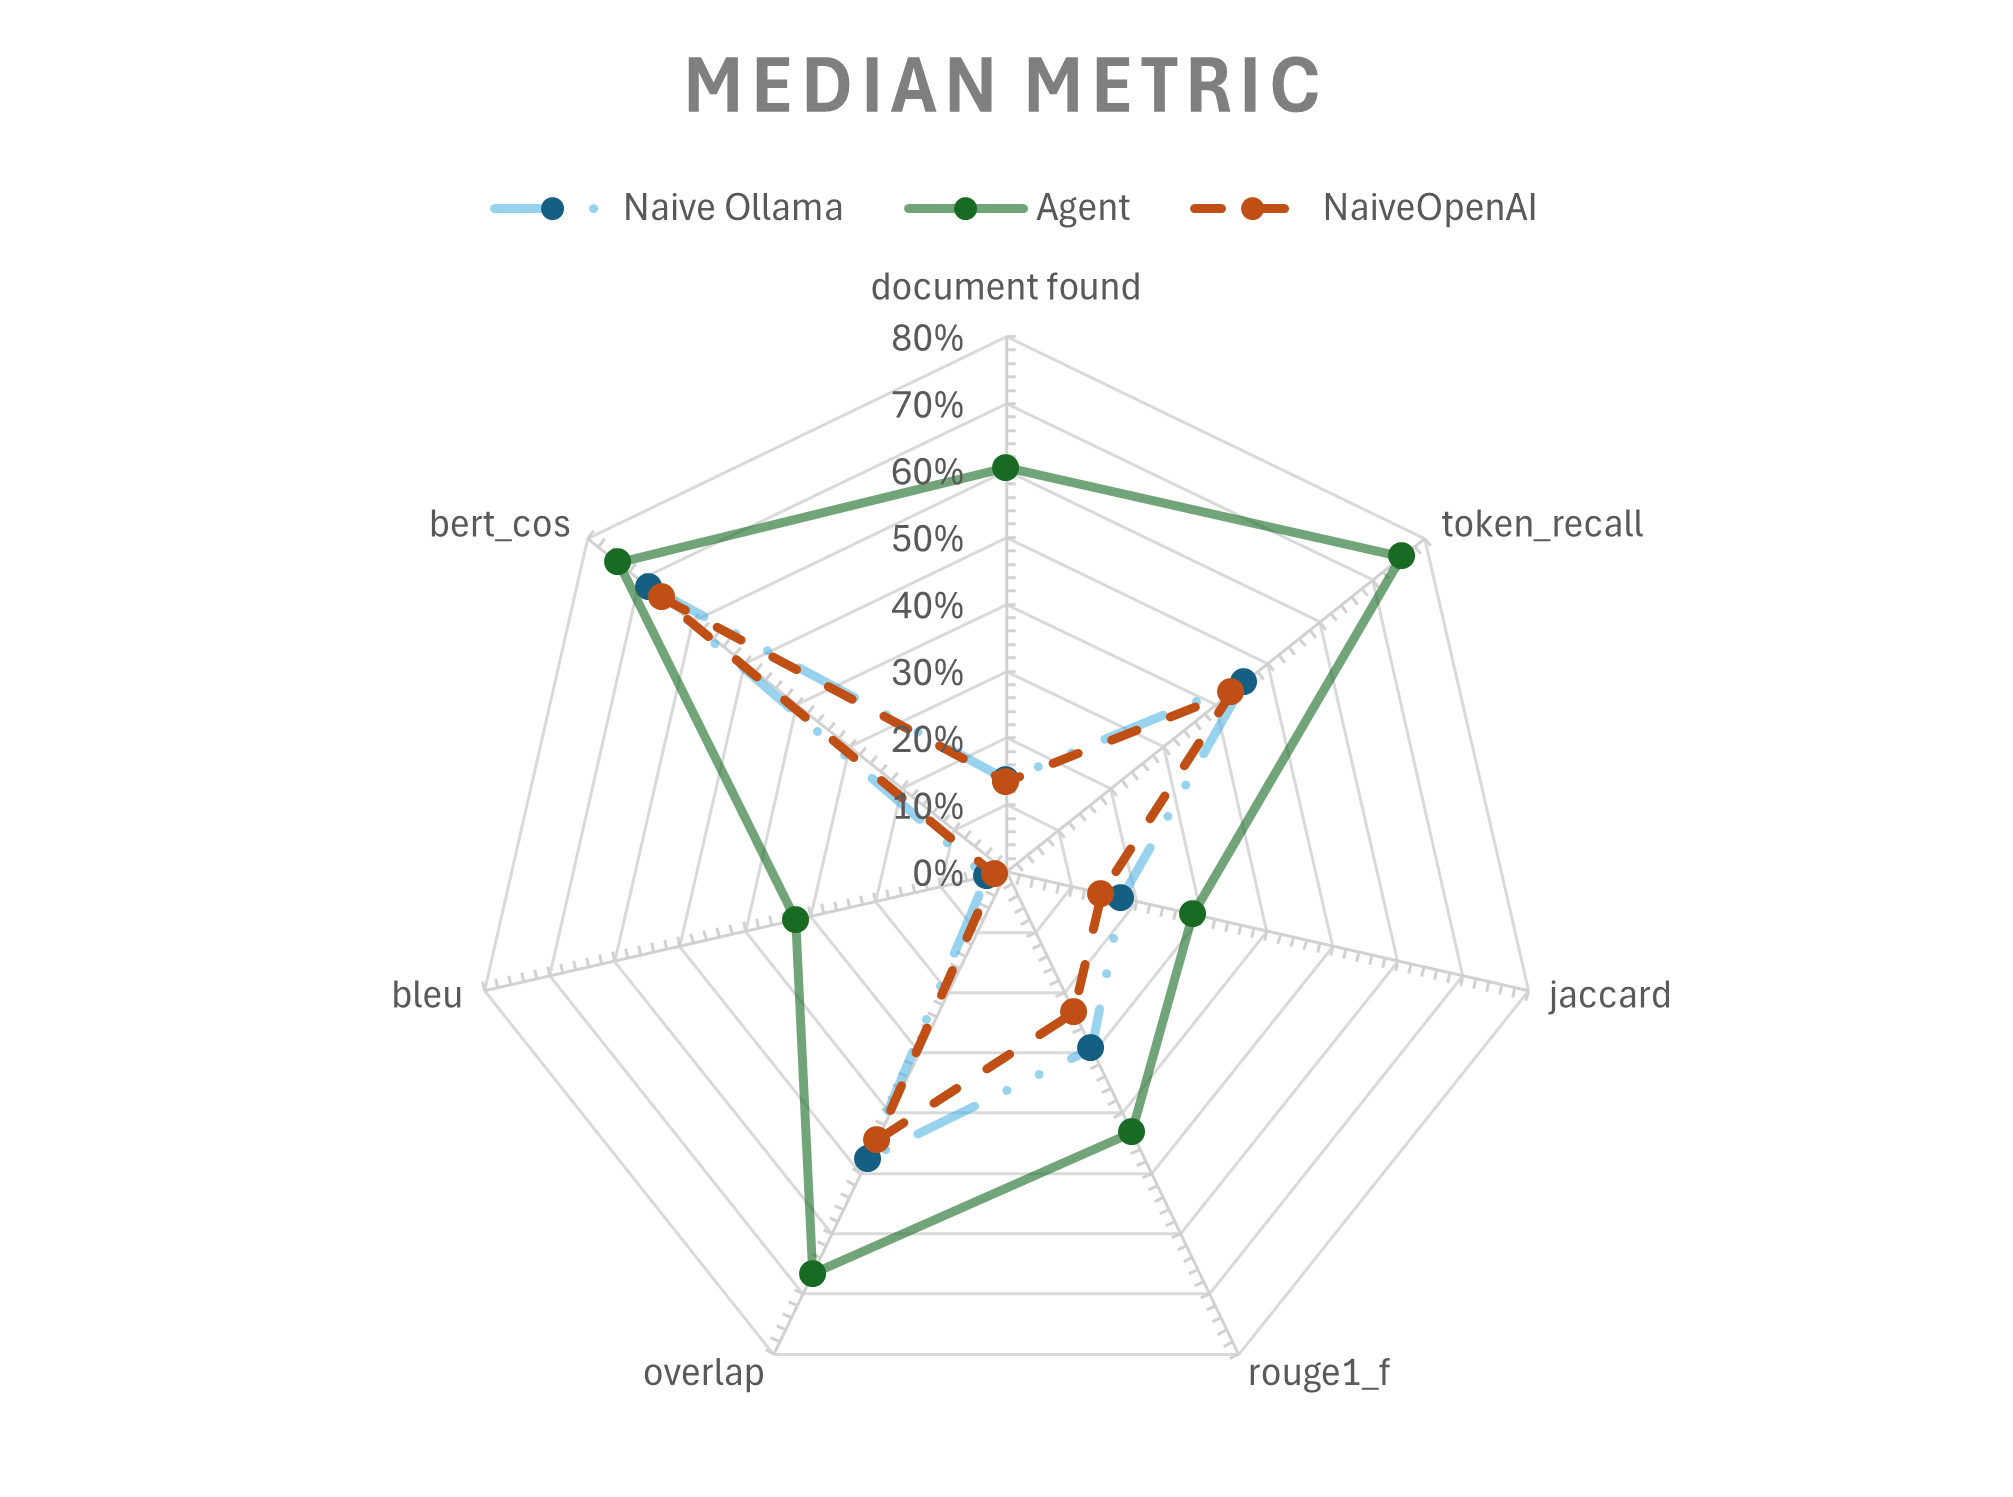
\includegraphics[width=0.75\linewidth]{Figures/Median Metric.png}
    \caption{Median Metric Scores}\label{fig:median-metric}
\end{figure}
According to Table~\ref{tab:agentopenai300-best-thresholds}, the metrics ranked by Youden's J statistic are: \textbf{Token Recall}, \textbf{Jaccard}, \textbf{ROUGE-1 F1}, \textbf{Overlap}, \textbf{BLEU}, and \textbf{\gls{BERT} cosine}. This ranking shows which thresholds are most effective for distinguishing correct from incorrect answers in this dataset. Token Recall attains the highest Youden's J value (52.3\%) because questions are specific, and correctness depends on including the correct content words, while surface fluency or paraphrase similarity is less critical. The -15\% trade-off observed in Table~\ref{tab:gain-loss-reference-median} reflects a deliberate threshold calibration: by optimizing for precision-oriented metrics (Jaccard, ROUGE-1), Token Recall is slightly reduced to prevent false positives, yielding a better overall classification balance. Conversely, \gls{BERT} cosine—which emphasizes sentence-level semantic similarity—performs worst here because many gold answers are short and exactness is essesntial. Jaccard performs well because it rewards coverage of relevant tokens relative to the union, serving as a useful proxy for answer completeness.

\begin{table}[htbp]
    \centering
    \begin{tabular}{l r r r  r r r}
        \hline
        Approach &  token recall & jaccard & rouge1 & overlap & bleu & \gls{BERT} cosine \\
        \hline
        Agentic ReAct (\gls{GPT}-5) &  -15\% & 27\% & 12\% & -3\% & 8\% & -13\% \\
        Naive \gls{RAG} (\gls{GPT}-5) &  -31\% & -1\% & -9\% & -16\% & 1\% & -38\% \\
        Naive \gls{RAG} (Qwen2.5) &  -26\% & 5\% & -8\% & -9\% & -1\% & -30\% \\
        \hline
    \end{tabular}
    \caption{Numerical differences when using agentic reference thresholds (Youden-optimized)\ref{fig:Youden-metric} versus median-based \ref{fig:median-metric} thresholds for classifying answers (positive values indicate gains).}
    \label{tab:gain-loss-reference-median}
\end{table}

Applying the agentic reference thresholds yields clear gains for \textit{Agent OpenAI} on \textit{Jaccard} (+27\%), \textit{ROUGE-1} (+12\%), and \textit{BLEU} (+8\%), with a trade-off in \textit{Token Recall} (\textminus 15\%). \textit{\gls{BERT} cosine} declines (\textminus 13\%) are expected give the stricter, token-accuracy oriented thresholding. The naive baselines exhibit broad declines—particulary in \textit{Token Recall} and \textit{\gls{BERT} cosine}—indicating that thresholds calibrated on higher-quality, better-retrieved agentic outputs do not gerenalize well to weaker systems.
\begin{figure}
    \centering
    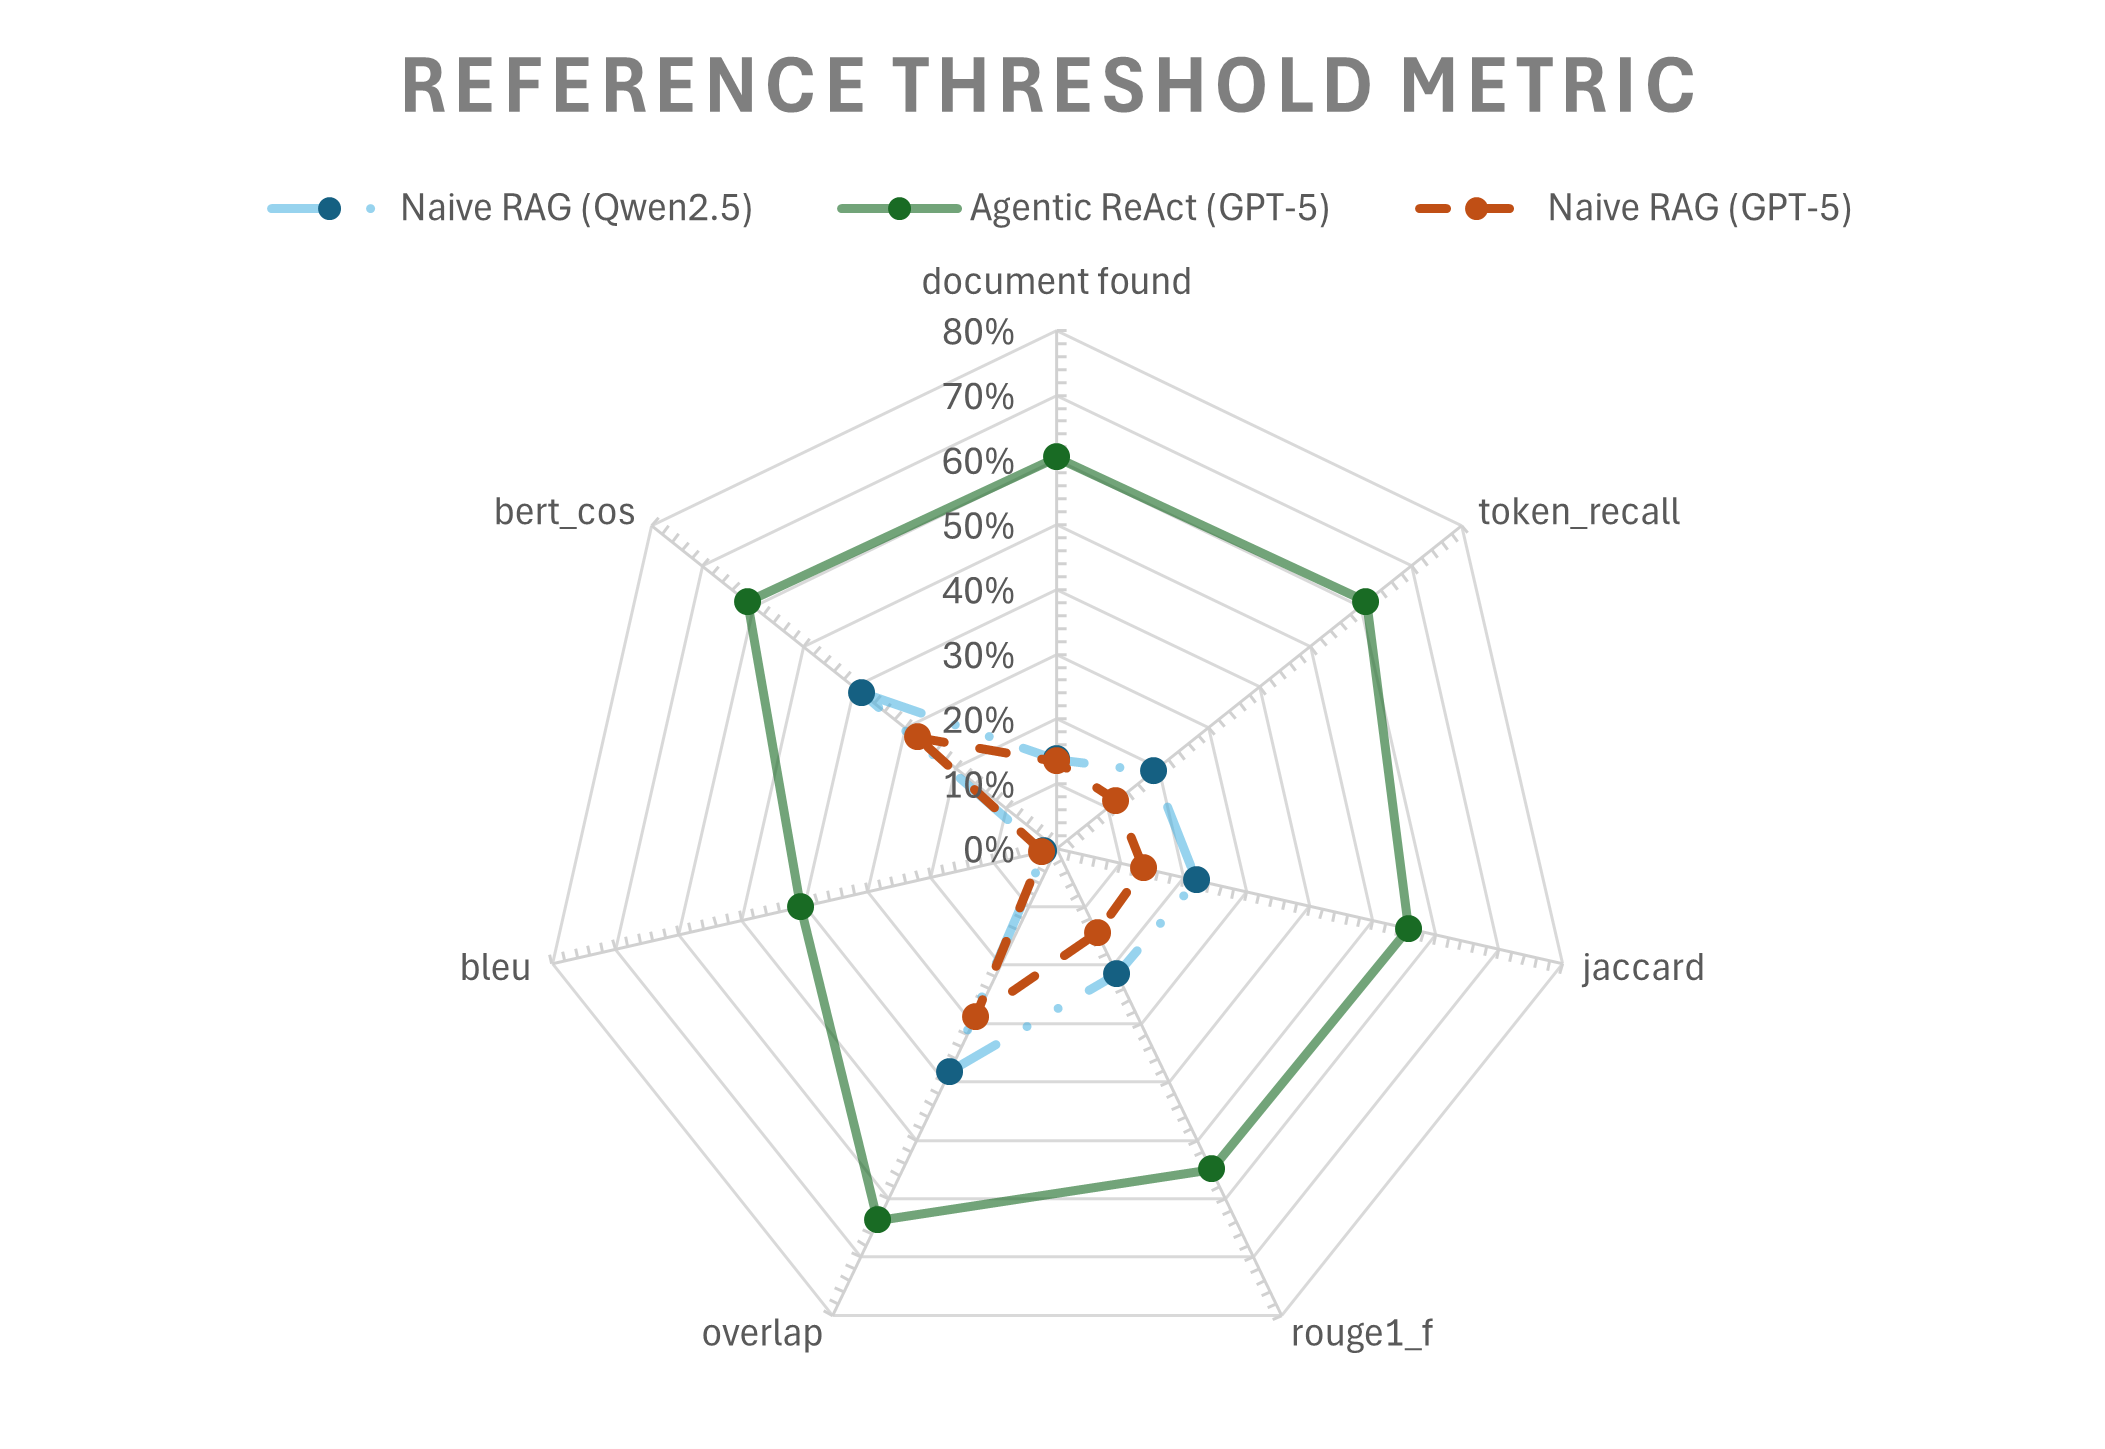
\includegraphics[width=0.75\linewidth]{Figures/Reference Threshold Metric.png}
    \caption{Agentic AI reference thresholds applied to all metrics of all important benchmarks}\label{fig:Youden-metric}
\end{figure}

Compared to the median-based thresholds, the agentic reference thresholds yield a more favorable profile for the \textit{Agent OpenAI} benchmark, boosting precision-oriented metrics (\textit{Jaccard}, \textit{ROUGE-1}, \textit{BLEU}) while sacrificing some recall (\textit{Token Recall}), while still maintaining a high score. This reflects the agent's ability to retrieve and synthesize relevant information more accurately, even if it occasionally omits less critical details. The naive baselines, however, do not benefit from this calibration, since their lower-quality outputs align less aligned well with the stricter criteria derived from the agentic system.

\begin{table}[htbp]
    \centering
    \begin{tabular}{l r r r r r r}
        \hline
        Approach & token recall & jaccard & rouge1f & overlap & bleu & \gls{BERT} cosine \\
        \hline
        Agentic ReAct (\gls{GPT}-5) & 61\% & 56\% & 55\% & 64\% & 41\% & 61\% \\
        Naive \gls{RAG} (\gls{GPT}-5) & 12\% & 14\% & 14\% & 29\% & 2\% & 28\% \\
        Naive \gls{RAG} (Qwen2.5) & 19\% & 22\% & 21\% & 38\% & 2\% & 39\% \\
        \hline
    \end{tabular}
    \caption{Share of answers passing Youden-optimized thresholds (Figure~\ref{fig:Youden-metric})}
    \label{tab:youden-metric-values}
\end{table}

Taken together with Figure~\ref{fig:Youden-metric}, these values show a pronounced separation between the agentic system and naive baselines under Youden-optimized criteria. The \textit{Agent OpenAI} workflow—plan, retrieve, observe/reflect, and answer—consistently classifies a much larger fraction of outputs as correct across metrics (e.g., 61\% Token Recall and 64\% Overlap), whereas naive pipelines lag substantially (e.g., Token Recall 12–19\%, Overlap 29–38\%). This demostrates the benefit of iterative reasoning and refinement over a single-pass naive RAG. This is also coupled by the fact that agentic RAG retrieves more documents correctly than the naive RAG system, as seen in Table~\ref{tab:doc-retrieved-by-source}.

\subsection{Cost and Latency Trade-offs}

Table~\ref{tab:naive-vs-agentic-tradeoffs} summarizes the cost and performance trade-offs between naive and agentic \gls{RAG} approaches. While naive \gls{RAG} is faster and cheaper (single retrieval + generation pass), agentic systems incur higher costs due to multiple reasoning and retrieval cycles. However, the significantly improved retrieval rate (60.4\% vs. 13.4\%–13.8\%) and answer quality justify this trade-off in mission-critical retrieval tasks.

\begin{table}[htbp]
    \centering
    \begin{tabular}{l r r r}
        \hline
        Approach & \gls{LLM} Calls/Query & Total Cost (300 Q) & Avg. Retrieval Rate \\
        \hline
        Naive \gls{RAG} (Qwen2.5) & 1--2 & 0 & 13.8\% \\
        Naive \gls{RAG} (\gls{GPT}-5) & 1--2 & \$5.07 & 13.4\% \\
        Agentic ReAct (\gls{GPT}-5) & 5--20 & \$18.35 & 60.4\% \\
        \hline
    \end{tabular}
    \caption{Comparative analysis of cost, latency, and retrieval effectiveness between naive and agentic \gls{RAG} approaches. Agentic systems require more \gls{LLM} calls but achieve substantially higher retrieval accuracy.}
    \label{tab:naive-vs-agentic-tradeoffs}
\end{table}

\section{Agentic Retrieval Across Multiple Collections}
\label{sec:agentic-retrieval-multiple}
In this experiment, the effectiveness of using multiple collections in Weaviate is evaluated and it is determined whether the agentic RAG system from Section~\ref{sec:agentic-test} can retrieve information distributed across multiple collections. The goal is to assess whether the agent can effectively navigate multiple data sources.

This is relevant in real-world scenarios where company information is distributed across separate databases or collections, each organized by department, project, or document type. For example, a media publisher may purchase content feeds from multiple providers. Each provider might expose its catalog through a Weaviate instance and sell API access rather than delivering raw data. With a successful agentic RAG system, the publisher can issue a single query across these sources, retrieve the most relevant passages and generate grounded answers for a news article.

To test this, two collections were set up in Weaviate. One collection is the same used in the previous experiment (Section~\ref{sec:expNaiveVsAgenticRAG}), containing 1,000 synthetic company documents. The second collection contains the LiHua-World dataset (Section~\ref{subsec:LiHua-World}).

For the \gls{QA} dataset, the 300 questions from the previous experiment (Section~\ref{sec:expNaiveVsAgenticRAG}) were combined with single-type questions from the LiHua-World dataset (637 in total) to match the synthetic setup. To migate collection bias and control cost, 200 random questions were sampled from each dataset, resulting 400 questions overall. The total cost was 13.56 dollars for input tokens and 3.11 dollars for output tokens, totaling 16.67 dollars.

For this test, results were recorded in \texttt{Agent\_OpenAI\_Mixed} and compared to the previous single-collection experiment \texttt{Agent\_OpenAI\_300}. Two subsets variants of the mixed dataset are also reported: \texttt{Agent\_OpenAI\_MixedLiHua} (LiHua-World questions only) and \texttt{Agent\_OpenAI\_MixedSynthetic} (synthetic company questions only).

To analyze the results, the percentage of questions for which the correct source document was retrieved is first examined, grouped by source document (Table~\ref{tab:doc-retrieved-by-source-mixed}). The mixed setting achieves higher retrieval rates than the single-collection setup. Part of this improviment likely reflects random variation in the sampled questions; notably, even the \emph{MixedSynthetic} split outperforms the single-collection setup. Despite potential sampling effects, the results indicate that the agent performs robustly when retrieving across multiple collections.
\begin{table}[htbp]
    \centering
    \begin{tabular}{l c}
        \hline
        Approach & Avg. Retrieval Rate \\
        \hline
    Agent\_OpenAI\_MixedLiHua & 93.0\% \\
    Agent\_OpenAI\_Mixed & 86.0\% \\
    Agent\_OpenAI\_MixedSynthetic & 80.5\% \\
    Agent\_OpenAI\_300 & 60.4\% \\
        \hline
    \end{tabular}
    \caption{Share of questions with the correct document retrieved, by result file}\label{tab:doc-retrieved-by-source-mixed}
\end{table}

\section{Optimization Using Summarization}
To optimize retrieval and generation performance, text summarization techniques were applied to the document corpus prior to indexing in Weaviate. The goal was to reduce document length while preserving essential information, facilitating more efficient embedding and retrieval.
This is particularly important for long documents where embedding models may truncate input or dilute semantic content.
Two summarization approaches tested are LexRank and BART-based abstractive summarization (see Section~\ref{sec:text-summarization} for details).
The original synthetic company documents (1000 files) were summarized using both techniques, resulting two new corpora: \texttt{Synthetic\_LexRank} and \texttt{Synthetic\_BART}. The source path to the unsummarized documents was retained for grounding answers in the Weaviate database.
Each summarized corpus was indexed in separate Weaviate collections employing the same schema as before (class \textit{Ficheiro} with properties \texttt{text} and \texttt{file\_path}, vectorized with \textit{all-MiniLM-L6-v2} embeddings). The agentic RAG system from Section~\ref{sec:agentic-test} was not evaluated because of budget constraints, and instead, the impact of summarization was tested with the purpose of optimizing storage, and denoising the database, to enable more efficient embedding and retrieval. Which is only required comparison between the naive RAG system from Section~\ref{sec:naive-rag-and-cot-baseline}.
Each summarization approach was evaluated through running the naive RAG pipeline (using \texttt{qwen2.5m} for generation) on the same 300-question benchmark in Section~\ref{sec:expNaiveVsAgenticRAG}. 

To take advantage of previous results, the best-performing naive RAG variant is used in Section~\ref{sec:naive-rag-and-cot-baseline} as a baseline: \texttt{weaviateNaive1\_300} (using hybrid search with \(\alpha=0.7\) and top-1 retrieval). Using the same evaluation metrics from Section~\ref{sec:metric-evaluation-quality}, the Youden's statistic metric thresholds from the most balanced benchmark, \texttt{Agentic React (\gls{GPT}-5)} are applied to compare performance across the three approaches: original, LexRank-summarized, and BART-summarized. The most important Youden's metrics analyzed are \textbf{Token Recall}, and \textbf{Jaccard}, which are used to best reflect the ability to retrieve the correct document and generate accurate answers in this experiment.
The results are presented in table~\ref{tab:document_retrieved_metrics_summarization}.

\begin{table}[t]
\centering
\caption{Document retrieval and summarization metrics}
\label{tab:document_retrieved_metrics_summarization}
\begin{tabular}{lrrr}
\hline
Approach & Avg. Retrieval Rate & token recall & jaccard \\
\hline
Agentic ReAct (\gls{GPT}-5)& 60.4\% & 61.1\%  & 55.7\%\\
LexRank & 33.6\% & 29.5\%  & 35.9\% \\
BART & 17.8\% & 3.0\% & 11.1\% \\
Naive \gls{RAG} (Qwen2.5) & 13.8\% & 19.1\% & 22.1\% \\
\hline
\end{tabular}
\end{table}

The results show that summarization techniques help reduce noise in the \gls{VD}, as Avg. Retrieval Rate increased for both summarization approaches compared to the naive RAG baseline (13.8\%): LexRank achieved 33.6\% and BART 17.8\%.
LexRank also improved Token Recall and Jaccard scores (29.5\% and 35.9\%, respectively), indicating that the extractive summaries preserved key information needed for accurate answering.
However, in the case of BART, Token Recall and Jaccard scores were markedly lower (3.0\% and 11.1\%, respectively), indicating althrough retrieval improved, the generated answers were less accurate. This suggests that BART's abstractive summarization may have omitted critical information for precise answering.
With these results, it is concluded that summarization of documents is a valuable step in a \gls{RAG} pipeline, functioning as a filter to reduce noise (irrelevant content).
However, the choice of summarization technique needs to be carefully considered: extractive methods like LexRank appear more effective as they preserve essential details, while abstractive methods like BART may risk losing important details.

 

\section{Cross-References Functionality}
\label{sec:crossrefs}
This section connects the thesis's core contribution—agentic semantic search with knowledge-graph traversal—to a concrete instantiation in Weaviate. We show how explicit cross-references act as traversable edges that both (i) enable deterministic multi-hop retrieval and (ii) serve as callable \enquote{tools} for an agent to plan and execute queries over the graph. We first recap the schema, then compare a hand-crafted traversal with an agentic ReAct workflow that uses the same edges programmatically.
To ground the agentic traversal results, we briefly recap the underlying Weaviate schema used throughout this chapter (cf. Figure~\ref{fig:weaviate_class}). The organizational model spans six classes—\textit{Fluxo} (workflow), \textit{Etapa} (stage), \textit{Entidade} (entity), \textit{Pasta} (folder), \textit{Ficheiro} (file), and \textit{Metadados} (metadata)—with named-vector properties for hybrid search (BM25 + vectors). Cross-references implement the navigation paths and serve as the "relational glue":
\begin{itemize}
    \item \textit{Fluxo} \(\rightarrow\) \texttt{hasEtapas}, \texttt{belongsToFicheiros}, \texttt{belongsToPastas}.
    \item \textit{Etapa} \(\rightarrow\) \texttt{belongsToFluxo}, \texttt{hasFicheiros}.
    \item \textit{Entidade} \(\rightarrow\) \texttt{hasPastas}, \texttt{hasFicheiros}.
    \item \textit{Pasta} \(\rightarrow\) \texttt{hasEntidades}, \texttt{hasFluxos}, \texttt{hasFicheiros}.
    \item \textit{Ficheiro} \(\rightarrow\) \texttt{belongsToMetadados}, \texttt{hasEtapas}, \texttt{hasPastas}, \texttt{hasEntidades}.
    \item \textit{Metadados} \(\rightarrow\) \texttt{hasFicheiros}, \texttt{hasEtapas}, \texttt{hasPastas}, \texttt{hasEntidades}.
\end{itemize}
These edges enable queries to traverse from workflows to stages to files, or from entities to folders to files and their associated metadata. In practice, hybrid search is used to find an entry point on any class, and references are followed to assemble grounded context for answering. As noted in the Weaviate documentation \cite{weaviate}, extensive cross-referencing can increase query latency; our agent therefore issues targeted traversals, following only the minimal set of edges required for each question.

\subsection{Latency and Scalability}
To complement the qualitative results above, we report the latency behavior of the system under increasing data sizes. The following figures summarize insertion and query times measured in our Weaviate setup. They illustrate that inserts scale near-linearly with the number of files and that query latency remains low and stable, even as collections grow.

% NOTE: Add the three PNG files below to the Figures/ folder with the same filenames.
% If your filenames differ, update the \includegraphics paths accordingly.
\begin{figure}[htbp]
    \centering
    % Three plots side by side
    \subfigure[Insert latency vs. files]{%
        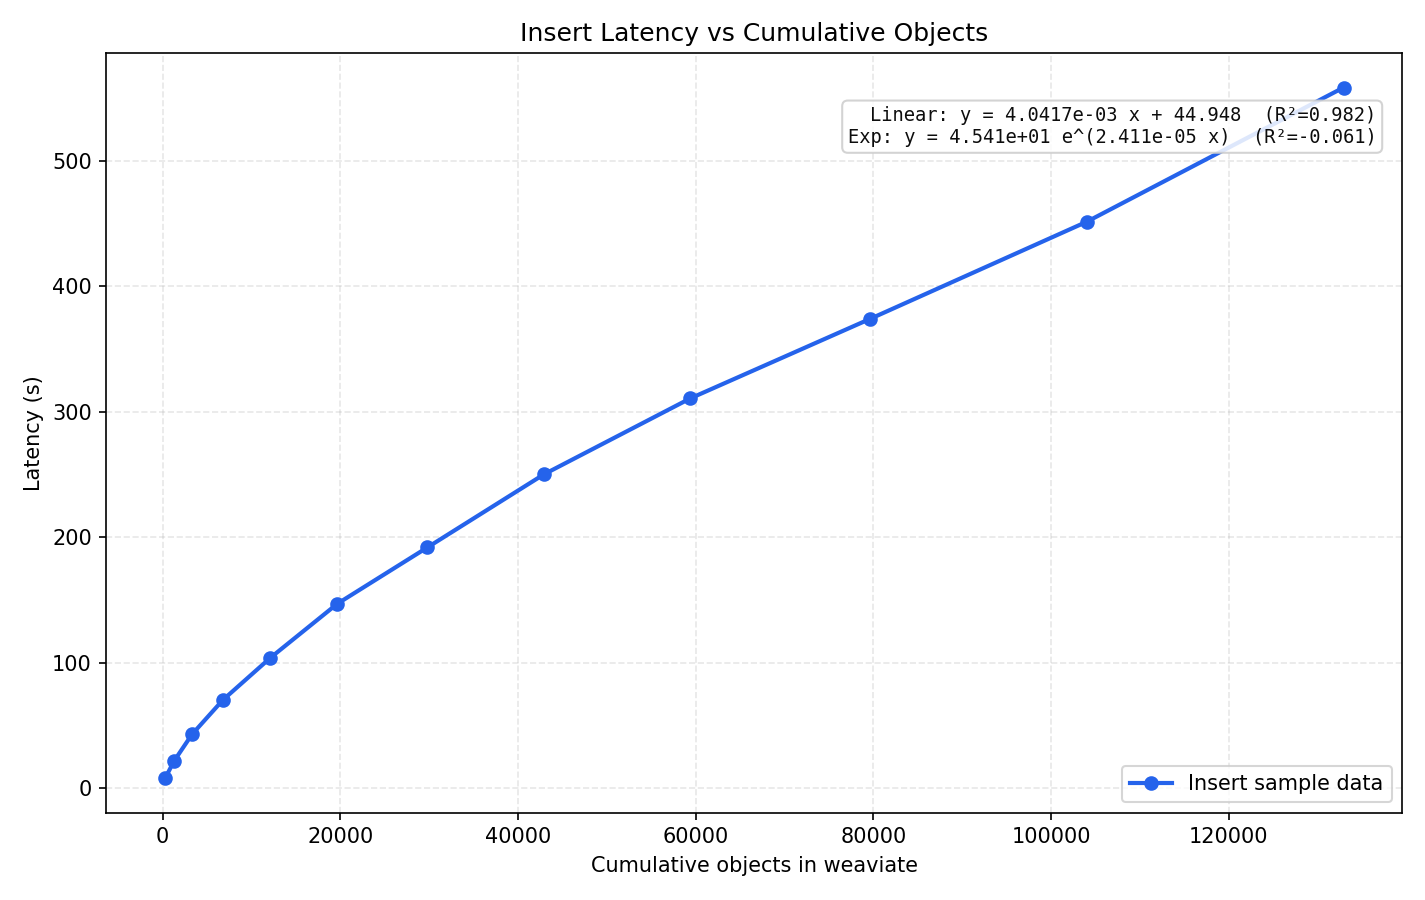
\includegraphics[width=0.32\linewidth]{Figures/insert_latency_vs_files.png}%
        \label{fig:insert-latency-vs-files}%
    }
    \hfill
    \subfigure[Query latency vs. files]{%
        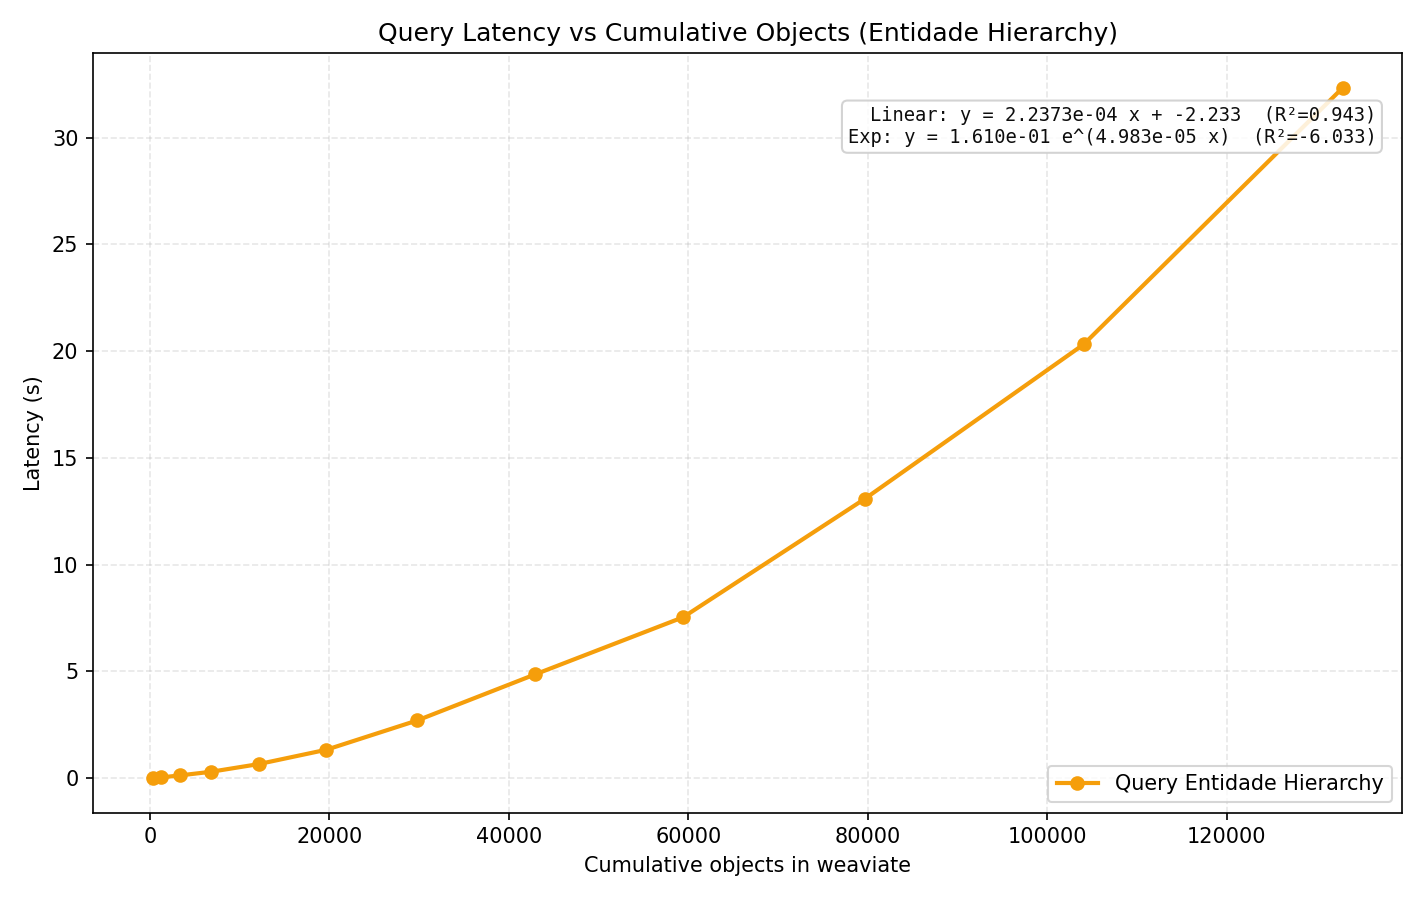
\includegraphics[width=0.32\linewidth]{Figures/query_latency_vs_files.png}%
        \label{fig:query-latency-vs-files}%
    }
    \hfill
    \subfigure[Global semantic search vs. total files]{%
        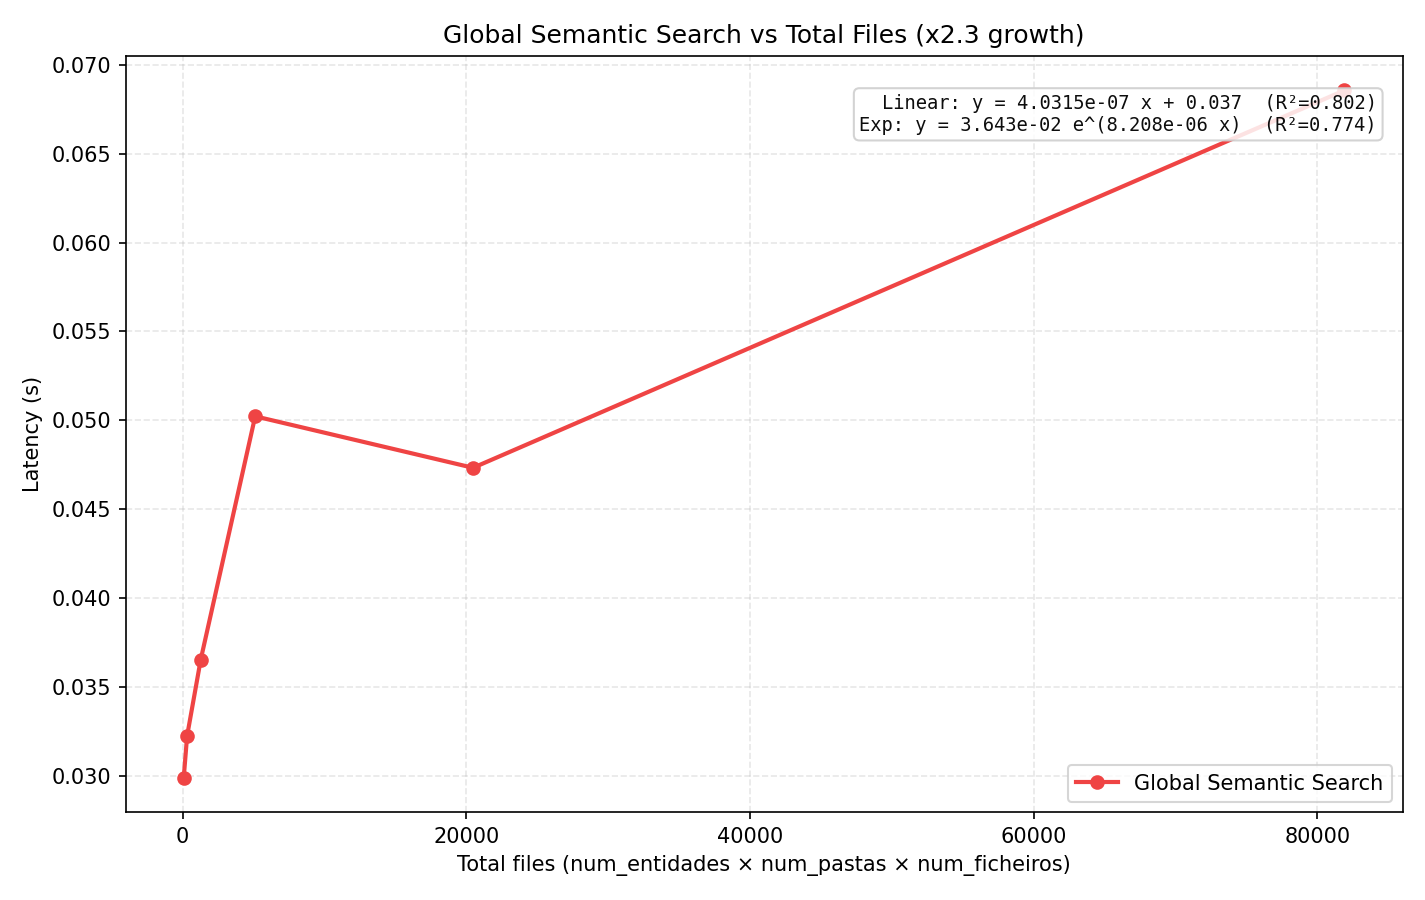
\includegraphics[width=0.32\linewidth]{Figures/semantic_latency_vs_files.png}%
        \label{fig:global-semantic-search-vs-total-files}%
    }
    \caption{Latency and scalability results measured on our Weaviate setup: (a) Insert Latency vs Number of Files (x577.5 growth, with linear and exponential trends and associated $R^2$); (b) Query Latency vs Number of Files comparing a structured traversal (Fluxo $\rightarrow$ Etapas) to a global semantic search; (c) Global semantic search latency as total files increase (x2.3 growth).}
\end{figure}

This section validates the practical value of cross-references by running two complementary tests on a compact, real-world–styled example: a structured Weaviate traversal demo and an \gls{ARAG} workflow that follows references via our developed \gls{MCP} server from Section~\ref{sec:weaviate-mcp-server}. 

 
\noindent\textbf{Realistic newsroom setting.} The example intentionally imitates how an international journalism company operates: frontline journalists and editors continuously file reports into the database according to the company's standards for maintaining organization in a highly scalable, dynamic environment. Requiring journalists to provide minimal structured metadata at submission time enables reliable traversal later. A typical filing flow is:
\begin{enumerate}
    \item inserts the document by filing the report as a \textit{Ficheiro} (with title, body, date);
    \item adds the topic in \textit{Fluxo} (storyline) and links the report to it;
    \item records people/organizations/countries in \textit{Entidade} and links them to the report (and stages when relevant);
    \item captures the event/tagging as an \textit{Etapa} (date, category, event) linked to the topic and the report.
\end{enumerate}

Cross-references transform the corpus from a flat, tag-based catalogue into a navigable graph. Unlike standard metadata tagging or hierarchical folder structures, graph organization is dynamic and traversable in high dimensions: edges encode who/what/where/when/etc. and enable deterministic multi-hop traversals. This design also benefits agentic systems by keeping context windows small—retrieving only the minimal set of linked nodes rather than entire files—thereby reducing token usage and latency. We adopt a newsroom scenario because editorial workflows align naturally with this structure: What is the news (\textit{Ficheiro})? To which storyline does it belong (\textit{Fluxo})? Who is involved (\textit{Entidade})? When did it occur (\textit{Etapa})? Keeping the example compact allows us to demonstrate how explicit edges yield grounded, auditable answers. Importantly, structure-aware retrieval improves explainability, trust, and compliance; it reduces ambiguity and accelerates handoffs in high-stakes environments. The schema mirrors the UML in Figure~\ref{fig:weaviate_class} and illustrates how explicit relationships complement semantic search, improving precision without sacrificing flexibility. In production deployments, schemas typically include additional classes and relationships; here we intentionally keep the model small to foreground the core functionality.

\subsection{Structured Demo in Weaviate (Deterministic Traversal)}
\label{subsec:weaviate-xref-structured}

We implemented a minimal newsroom graph using UML classes from Figure~\ref{fig:weaviate_class} that mirrors a common editorial workflow using four classes and cross-references. This graph is dynamic and extensible—edges and nodes can be added as needed to capture new relationships. We omitted the \textit{Pasta} (Folder) class because it is not required for this example. 
The four classes and their key properties/references are:
\begin{itemize}
    \item \textbf{Entidade} (entity): countries, people, organizations; \texttt{hasReports} \(\rightarrow\) \textit{Ficheiro}
    \item \textbf{Ficheiro} (report/file): title, body, date; \texttt{hasEntidades} \(\rightarrow\) \textit{Entidade}, \texttt{belongsToFluxo} \(\rightarrow\) \textit{Fluxo}, \texttt{triggersEtapas} \(\rightarrow\) \textit{Etapa}
    \item \textbf{Fluxo} (topic/storyline): name, description; \texttt{hasStages} \(\rightarrow\) \textit{Etapa}, \texttt{hasReports} \(\rightarrow\) \textit{Ficheiro}
    \item \textbf{Etapa} (stage/event): name, date, description, category; \texttt{belongsToFluxo} \(\rightarrow\) \textit{Fluxo}, \texttt{aboutReports} \(\rightarrow\) \textit{Ficheiro}, \texttt{aboutEntities} \(\rightarrow\) \textit{Entidade}
\end{itemize}

The demo starts by illustrating how a journalist reports: they insert their document and then add information around it—\textit{Entidade} (who is involved), \textit{Fluxo} (topic/storyline), and \textit{Etapa} (event/date). It then inserts one topic (\enquote{Russia vs Ukraine War}), a report (\enquote{Drone attack hits military base}), entities (\enquote{Russia}, \enquote{Ukraine}, and a journalist \enquote{Jane Doe}), and a stage (\enquote{Destruction of a military base}, category \texttt{war\_crime}). It links objects along the graph edges so traversal is possible.

\begin{quote}
\enquote{Ficheiro.title}: \enquote{Drone attack hits military base} \quad \enquote{Ficheiro.date}: \enquote{2024-07-12T00:00:00Z}\\
\enquote{Fluxo.name}: \enquote{Russia vs Ukraine War}\\
\enquote{Entidade.name}: \enquote{Russia}, \enquote{Ukraine}, \enquote{Jane Doe} (role: \enquote{Journalist})\\
\enquote{Etapa.name}: \enquote{Destruction of a military base} \quad (category: \enquote{war\_crime}; date: \enquote{2024-07-12T00:00:00Z})
\end{quote}

For the complete insertion listing with all fields and cross-references, see Appendix~\ref{chapter:appendixA}, Section~\ref{app:newsroom-insertion}.

\noindent\textit{In practice.} This structure enables immediate, deterministic traversals that answer common newsroom questions:
\begin{itemize}
    \item \textbf{Topic status:} Load the \textit{Fluxo}, follow \texttt{hasStages} and \texttt{hasReports}, sort stages by \texttt{date} client-side, and return the latest stage and report count.
    \item \textbf{Latest war crime:} From the \textit{Fluxo}, traverse \texttt{hasStages} and filter \textit{Etapa} by \texttt{category = war\_crime}; pick the most recent by \texttt{date}.
    \item \textbf{Who reported?:} From the latest \textit{Etapa}, follow \texttt{aboutReports} $\rightarrow$ \textit{Ficheiro} and then \texttt{hasEntidades} to extract people whose \texttt{role} contains \enquote{Journalist}.
    \item \textbf{Start anywhere:} Use hybrid search (BM25 + vectors) on any class to find an entry point (e.g., report, entity, stage), then follow references to aggregate the full context.
\end{itemize}


Process steps mirror the newsroom workflow outlined above, so we omit restating them for brevity. Practically, this structured linking improves retrieval: finding any one of the linked objects (e.g., the report, topic, entity, or stage) is sufficient for the system to follow references and surface all related context. This reduces reliance on text-only retrieval and enables fast, explainable navigation across the repository.

\noindent\textit{Outcome (qualitative).} Because relationships are explicit, these questions are answered by graph navigation rather than free-text similarity. For the inserted example, \texttt{topic\_status} returns the most recent stage; \texttt{latest\_war\_crime} yields the staged event tagged as \texttt{war\_crime}; and \texttt{reporters\_for\_latest\_stage} surfaces the journalist linked to the report that triggered that stage. Hybrid search provides a flexible fallback and a cross-class discovery view, but the multi-hop answers are grounded by references.
Although illustrative, the foregoing results are obtained with manually engineered queries—a capability long established in relational database systems. The next subsection evaluates whether an autonomous agent can exploit these references programmatically. Agent-mediated traversal of references is comparatively more novel and potentially more powerful, as it enables autonomous planning and execution over the graph rather than reliance on fixed, hand-coded traversals. 
\subsection{Agentic RAG over Cross-References (Tool-using ReAct)}
\label{subsec:agentic-xref}
To test whether an agent can leverage cross-references programmatically, we implemented a ReAct-style agent using OpenAI SDK that connects to Weaviate via the \gls{MCP} server developed in this work (Section~\ref{sec:weaviate-mcp-server}). The agent uses a system prompt instructing it to request \enquote{weaviate-origin} and \enquote{weaviate-follow-ref} tools when it needs data and to extract key fields from results. It maintains a persistent session (SQLite) and includes retry/backoff logic.

The agent is asked the same three questions as in the structured demo:
\begin{enumerate}
    \item \enquote{How is the war on Russia and Ukraine?}
    \item \enquote{What is the latest war crime?}
    \item \enquote{Who reported?}
\end{enumerate}
Under the hood, the agent plans, issues a reference-origin query (e.g., load the \textit{Fluxo}), follows references (e.g., \texttt{hasStages} \(\rightarrow\) \textit{Etapa}, \texttt{aboutReports} \(\rightarrow\) \textit{Ficheiro}, \texttt{hasEntidades} \(\rightarrow\) \textit{Entidade}), inspects properties (\texttt{date}, \texttt{category}, \texttt{role}), and produces a concise, grounded answer. Ordered navigation traces for these questions are provided in Appendix~\ref{app:agentic-navigation-traces}, and a graph visualization of this example is provided in Appendix~\ref{fig:schema-example}.
Connectivity checks, Windows-specific event loop policy, and transport selection (stdio or HTTP) are handled by the script.

\noindent\textit{Outcome (qualitative).} On the inserted example, the agent retrieves the topic status, identifies the most recent war-crime stage, and extracts the reporter by following references, matching the deterministic traversal results via tool calls. This validates that cross-references are usable not only by handcrafted queries but also by an autonomous planner that reasons over the graph.

\subsection{Takeaways and Scope}
Cross-references provide the \emph{relational glue} required for multi-hop questions: latest-by-date, filtered-by-category, \enquote{who caused/reported what}, and similar patterns. In the structured setting (Section~\ref{subsec:weaviate-xref-structured}), answers are repeatable and explainable because they follow explicit edges. In the agentic setting (Section~\ref{subsec:agentic-xref}), the same edges become \emph{tools} that an \gls{LLM} can call to plan-and-execute traversals. While we did not run a large-scale accuracy benchmark here ---as none are available for complex agentic structure retrieval, and a synthetic benchmark is over the thesis's budget --- these tests demonstrate functional correctness and integration readiness: the schema supports reference navigation, and the agent can exploit it to produce grounded, auditable answers. Results are in Appendix~\ref{app:agentic-navigation-traces}.


% Finally, the summarization techniques were also evaluated in the mixed dataset from Section~\ref{sec:agentic-retrieval-multiple}, combining both LiHua-World and synthetic company questions. The same naive RAG pipeline (using \texttt{qwen2.5m} for generation) was run on the mixed 400-question benchmark, using the same Weaviate collections with summarized documents. In this case the collections were merged in to one, as the decision making of a agent is not relevant in this experiment. The goal of this experiment, is evaluating the impact of summarization techniques in a mixed dataset scenario.

% The results are presented in table~\ref{tab:document_retrieved_metrics_mixed}.
% \begin{table}[t]
% \centering
% \caption{Document retrieval and summarization metrics using mixed dataset from Section~\ref{sec:agentic-retrieval-multiple}}
% \label{tab:document_retrieved_metrics_mixed}
% \begin{tabular}{lrrr}
% \hline
% Approach & Avg. Retrieval Rate & token recall & jaccard \\
% \hline
% MixedLiHua & 46.5\% & 15.8\% & 1.27\% \\
% MixedTotal & 39.4\% & 24.6\% & 19.3\% \\
% LexRank & 33.6\% & 29.5\%  & 35.9\% \\
% MixedSynthetic & 33.0\% & 31.5\% & 33.5\% \\
% \hline
% \end{tabular}
% \end{table}

% The results show that summarization techniques need to be carefully considered. As the Lihua-World benchmark, Avg. Retrieval Rate is high, the answer quality is poor. This happens because the Lihua-World dataset, is dialogues snippets, of a fictional story. Where details are more hidden. Therefore, LexRank summarization ended up removing 